\documentclass[a4paper,12pt]{article} % тип документа

% report, book

% Рисунки
\usepackage{graphicx}
\usepackage{wrapfig}
\usepackage{mathtext}
\usepackage[left=2cm,right=2cm,
    top=2cm,bottom=2cm,bindingoffset=0cm]{geometry}

\usepackage{hyperref}
\usepackage[rgb]{xcolor}
\hypersetup{				% Гиперссылки
    colorlinks=true,       	% false: ссылки в рамках
	urlcolor=blue          % на URL
}

%  Русский язык
\usepackage[T2A]{fontenc}			% кодировка
\usepackage[utf8]{inputenc}			% кодировка исходного текста
\usepackage[english,russian]{babel}	% локализация и переносы
\addto\captionsrussian{\def\refname{Список используемой литературы}}


% Математика
\usepackage{amsmath,amsfonts,amssymb,amsthm,mathtools} 
\usepackage{titlesec}
\titlelabel{\thetitle.\quad}

\usepackage{wasysym}
\title{3.3.4 Эффект Холла в полупроводниках}
\date{}

\begin{document}

\begin{center}
\textsf{\textbf{3.3.4 ЭФФЕКТ ХОЛЛА В ПОЛУПРОВОДНИКАХ}}
\end{center}

\textbf{Цель работы:} измерение подвижности и концентрации носителей заряда
в полупроводниках.

\textbf{В работе используются:} электромагнит с регулируемым источником питания; вольтметр; амперметр; миллиамперметр; миллитесламетр; источник питания, образцы легированного германия.

Перед выполнением работы необходимо ознакомиться с основами элементарной теории движения носителей заряда в металлах и полупроводниках (п. 4 введения к разделу).

В работе изучаются особенности проводимости полупроводников в
геометрии мостика Холла. Ток пропускается по плоской полупроводниковой пластинке, помещённой в перпендикулярное пластинке магнитное
поле. Измеряется разность потенциалов между краями пластинки в поперечном к току направлении. По измерениям определяется константа
Холла, тип проводимости (электронный или дырочный) и вычисляется концентрация основных носителей заряда на основе соотношения:
\begin{equation}
R_H = \frac{1}{nq},
\end{equation}
где $n$- концентрация основных носителей заряда, $R_H$ -постоянная Холла, $q$ - заряд носителя.

\textbf{Экспериментальная установка}
\begin{figure}[h!]
\begin{center}
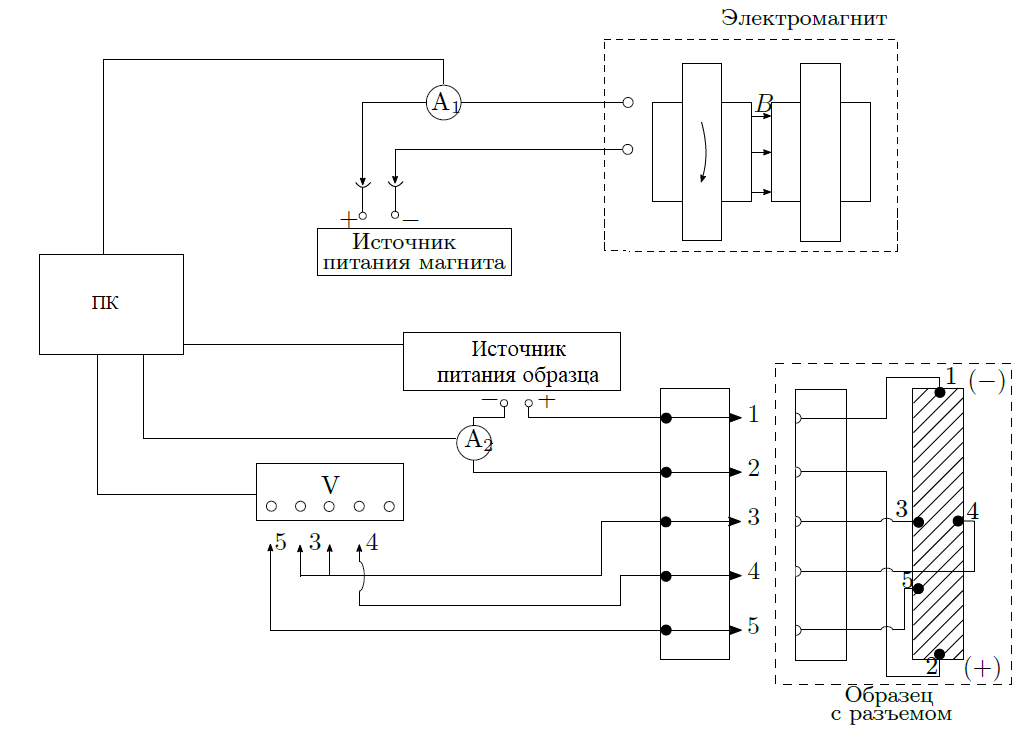
\includegraphics[width=0.76\textwidth]{Установка}
\caption{Схема установки для исследования эффекта Холла в полупроводниках} \label{установка}
\end{center}
\end{figure} 

Электрическая схема установки для измерения ЭДС Холла представлена на рис. \ref{установка}. В зазоре электромагнита (рис. \ref{установка}а) создаётся постоянное
магнитное поле, величину которого можно менять с помощью регулятора источника питания электромагнита. Ток питания электромагнита измеряется внешним амперметром А1.
Направление тока в обмотках электромагнита меняется переключением
разъёма К1.

Градуировка электромагнита (связь тока с индукцией поля) проводится при помощи миллитесламетра на основе датчика Холла.

Прямоугольный образец из легированного германия, смонтированный в специальном держателе (рис. \ref{установка}б), подключается к источнику питания образца. При замыкании ключа К2 вдоль длинной стороны образца
течёт ток, величина которого регулируется на источнике питания образца и измеряется миллиамперметром А2.

В образце, помещённом в зазор электромагнита, между контактами 3
и 4 возникает разность потенциалов 34, которая измеряется с помощью
вольтметра V.

Контакты 3 и 4 вследствие неточности подпайки могут лежать не на
одной эквипотенциали. Тогда напряжение между ними связано не только с эффектом Холла, но и с омическим падением напряжения вдоль
пластинки. Исключить этот эффект можно, если при каждом значении тока через образец измерять напряжение между точками 3 и 4 в отсутствие магнитного поля. При фиксированном токе через образец это дополнительное к ЭДС Холла напряжение $U_0$ остаётся неизменным. От него следует (с учётом знака)
отсчитывать величину ЭДС Холла:
\begin{equation}
U_\perp = U_{34} - U_0
\end{equation}
При таком способе измерения нет необходимости проводить повторные
измерения с противоположным направлением магнитного поля.

По знаку $U_\perp$ можно определить характер проводимости — электронный или дырочный. Для этого необходимо знать направление тока в
образце и направление магнитного поля.

Измерив ток $I$ в образце и напряжение $U_{35}$ между контактами 3 и 5
в отсутствие магнитного поля, можно, зная параметры образца, рассчитать проводимость материала образца по формуле
\begin{equation}
\rho_0=\frac{U_{35}ah}{Il}
\end{equation}
где $l$ — расстояние между контактами 3 и 5, $a$ — ширина образца, $h$ —
его толщина.


\begin{center}
\textsf{\textbf{ЗАДАНИЕ}}
\end{center}
В работе предлагается исследовать зависимость ЭДС Холла от величины магнитного поля при различных значениях тока через образец для
определения константы Холла; определить знак носителей заряда и проводимость материала образца.


\begin{enumerate} 
	\item Работа будет состоять из 4 частей: градуировка электромагнита, основной эксперимент (эфект холла), определение знака носителей, измерение удельной проводимости.
  \item Соберите установку согласно схеме на рис. \ref{установка}, подключите к вольтметру контакты 3 и 4.
  \item Запустите программу <<Эффект Холла>>
  \item Введите фамилие в поле <<Введите фамилию>>, нажмите клавишу ENTER.
  
  \item Для проведения градуировки электромагнита ознакомьтесь с устройством и принципом работы измерителя магнитной индукции ATE-8702. Техническое описание (ТО) расположено на установке.
  Включите измеритель индукции кнопкой <<POWER>>; через 2-3 секунды последовательным нажатием кнопки <<MODE>> установите режим измерения в постоянном поле  <<$a_1$>> (см. рис. 2 ТО).
  
  Снимите защитный колпачок с сенсорной головки датчика и коснитесь головкой поверхности магнита в зазоре.
  
  Для удержания показаний дисплея нажмите кнопку <<HOLD>>; повторное нажатие этой кнопки возвращает прибор в режим измерений.
  
  \item Установите ручки регулировки источника питания электромагнита в минимальное положение и нажмите на кнопку <<Градуировка электромагнита>>. Для начала эксперимента нажмите кнопку  <<Старт>>.
  
   Получите калибровочную кривую электромагнита: измерьте магнитную индукцию миллитесламетром, полученное значение введите в поле  <<Индукция>>, нажмите клавишу ENTER, плавно измените ток питания электромагнита. Повторите для 15-20 значений тока питания электромагнита.
  \item После окончания калибровки выйдите в меню программы с помощью клавиши  <<Меню>>. Перейдите к выполнению основного эксперимента кнопкой <<Основной эксперимент>>.
  \item Введите $a$ в поле <<Введите a>>, нажмите клавишу ENTER. Установите ручки регулировки источника питания электромагнита в минимальное положение, нажмите кнопку <<Старт>>. Снимите 15 точек, затем, остановив процесс кнопкой  <<Стоп>>, измените ток на источнике питания электромагнита. Запустите получение данных кнопкой  <<Новое напряжение>>. Повторите для 10-12 значений тока на источнике питания электромагнита.
  \item После окончания основного эксперимента выйдете в основное меню программы кнопкой  <<Меню>>. Перейдите к определению знаку носителей заряда кнопкой <<Основной эксперимент>>.
  \item Определите знак носителей заряда в образце. Для этого необходимо
знать направление тока через образец, направление магнитного поля
и знак ЭДС Холла.

Направление тока в образце показано знаками  <<+>> и  <<->> на рис. \ref{установка}.
Направление тока в обмотках электромагнита при установке разъёма $K_1$ в положение 1 показано стрелкой на торце магнита. 

Измерьте разность потенциалов без магнитного поля (установите ручки регулировки источника питания электромагнита в минимальное положение, нажмите кнопку  <<Без поля>>). Подайте небольшое напряжение на электромагнит, нажмите кнопку  <<С полем>>. Определите характер проводимости образца (дырочный или электронный). 

\item Выключите источник питания электромагнита, перейдите в основное меню программы кнопкой  <<Меню>>. Перейдите к измерению удельной проводимости соответствующей кнопкой.
\item Удалите держатель с образцом из зазора электромагнита; подключите к клемма  <<U>> и  <<0>> вольтметра провода 3 и 5; введите параметры образца в соответствующие поля (после ввода обязательно нажать клавишу  <<ENTER>>). Введите $L$  в поле <<Введите L>> и $l$ в поле <<Введите l>>, нажмите кнопку  <<Старт>>.
\item Перейдите в основное меню программы. Для получения графиков и постоянных из эксперимента нажмите на кнопку  <<Обработка данных>>. 
\item Разберите установку, все полученные данные и графики хранятся в папке с вашей фамилией, сохраните их себе, например, на флешку.
  
\end{enumerate}

\end{document}